% !TEX encoding = UTF-8 Unicode
\documentclass[]{llncs}
\usepackage[utf8]{inputenc}

\usepackage{graphicx}
\usepackage{ifpdf}

%\usepackage{fullpage}
%\usepackage{amsmath}
%\usepackage{amssymb} 
%\usepackage{amsthm} 
% \usepackage{hyperref}
% \usepackage{float}
% \theoremstyle{definition} 
% \usepackage{graphicx}
% \newtheorem{theorem}{Theorem}[subsection]
% \newtheorem{lemma}{Lemma}[subsection]
% \newtheorem{definition}{Definition}[subsection]
% \newtheorem{conjecture}{Conjecture}[subsection]
% \newtheorem{corollary}{Corollary}[subsection]
% \renewcommand{\intextsep}{0.1in}

% \ifpdf
% \usepackage[pdftex]{graphicx}
% \else
% \usepackage{graphicx}
% \fi

\newcommand{\NOTE}[1]{{\bf NOTE: {#1}}}

\usepackage{color}
\newcommand{\TODO}[1]{{\textcolor{blue}{ToDo: {#1}}}}



\title{\bf Eagle Knights 2017: Small Size League\\ Team Description Paper}
\author{Edgar Granados, Diego Pozo, Mariana Hernández, Erick Zetina, Ruiciro Rivera and Marco Morales}
\institute{Robotics Laboratory, Department of Digital Systems, ITAM\\
Río Hondo 1, Ciudad de México, 01080, México}

\date{}
\begin{document}

\ifpdf
\DeclareGraphicsExtensions{.pdf, .jpg, .tif, png}
\else
\DeclareGraphicsExtensions{.eps, .jpg}
\fi

\maketitle
\begin{abstract}
In this paper we describe the architecture of our RoboCup Small Size League 2017 team. Both, our hardware and software have evolved since 2014 with major updates in 2016 and 2017. In hardware, we are now using brushless motors, new computational components based on a micro-controller and an FPGA, and WiFi communications. In software, we have a modular system based on ROS with improvements in obstacle avoidance and behaviors.
\keywords{Small Size League, RoboCup, ROS}
\end{abstract}

\section{Introduction}

Here, we present the Eagle Knights system to participate in the RoboCup 2017. The RoboCup \cite{robocup-ssl-rules} is an international joint project to advance research on artificial intelligence and robotics through a grand challenge: design a robotics soccer team able to defeat the FIFA world champion by 2050. The Small Size League takes this challenge by promoting research on multi-agent cooperation and control. Two teams of six mobile robots up to 18 cm in diameter and 15 cm in height play soccer on a 9 m by 6 m carpeted soccer field. Aerial cameras placed 4m above the playing surface send video signals to a shared vision system\cite{zlbwv-sslvtsvsftrcssl-RoboCup-2009} that estimates the position of the robots and of the ball on the field. This information is then passed to a decision system that produces the control commands that are sent to each of robot in the team through a wireless link. An external referee box indicates the state of the game to the central computer. 

% \TODO{Check if we still are compliant with 2017 rules, number of robots, size, lengths of soccer field, type of carpet, distance to aerial cameras, shared vision system, referee box}

The Eagle Knights SSL team was founded in 2003 and participated officially for the first time in Robocup 2005. Our team was the first Latin American team consistently obtaining top results in all its regional RoboCup participation, 3rd and 2nd place in US Open 2003 and 2004, respectively, and 1st place in Latin American Open 2004 and 2005. We have also participated in the following RoboCup competitions: Osaka, Japan 2005; Bremen, Germany 2006; Atlanta, USA 2007; Suzhou, China 2008; Graz, Austria 2009 ;  Singapore 2010; Istanbul, Turkey 2011; and Mexico City, Mexico 2012. In 2016 we pushed our systems and this year we present a much improved team. We are working to have a competitive team again within the next year.

\begin{description}
	\item[Eagle Knights official website] http://robotica.itam.mx/ssl
	\item[Qualification video URL] http://robotica.itam.mx/videos/EK-qualification-ssl-2017.mp4
\end{description}

% \TODO{Make sure the video is put in the link mentioned above}

\section{Team Constitution}

Our team is integrated by Faculty and undergraduate students from ITAM (Instituto Tecnológico Autónomo de México).
\begin{itemize}
\item {\bf Faculty advisor} Prof. Marco Morales, PhD.
\item {\bf College student members} 
Edgar Alejandro Granados Osegueda,
Diego Pozo Barruel,
Mariana Raquel Hernández Rocha,
Brandon Francisco Hernández Troncoso,
Erick Zetina Muciño,
Ruiciro Rivera Serrano, and
Humberto Isaac Téllez Benítez

%\item {\bf Hardware group}
%\item {\bf Software group}
%\item {\bf Administration and Public Relations.}
\end{itemize}


\section{Overview of the Eagle Knigths Small Size League System EK-bots}

We currently have two robots that satisfy the constraints set in the SSL rules, being capable of easily producing more for a complete team:
\begin{description} 
	\item [The height] of each robot is 147 mm
	\item [The maximum diameter] of its projection to the ground is 170 mm
	\item [The maximum percentage of ball coverage] is 15\%. 
\end{description}

% \TODO{verify the dimensions of our robots (rules say max height 150mm, max diameter 180mm, max coverage 20\%)}

As shown in Fig.~\ref{fig:eagle-knights-architecture} we have built a distributed system based on ROS that includes the following ROS nodes: Vision, Referee Box, Strategy, Action/Motion Planning, Trajectory, and Communications. A vision node is a wrapper for the SSL vision system. A referee box node is a wrapper for the SSL referee box. A strategy node defines the actions for each player according to the state of the game, the role of the player, and the configurations of all the robots and the ball. An action/motion planning node defines the next position for each robot according to the action it is performing and the obstacles (other robots) in the environment. A trajectory node computes the velocity commands to be sent to each robot based on their current pose and goal configurations. A communications node receives velocity commands for the robots and passes them through an XBee WiFi Arduino shield. A monitor node allows us to visualize the status of the robots and provide manual controls for testing.

\begin{figure}[htb]
	\centering
	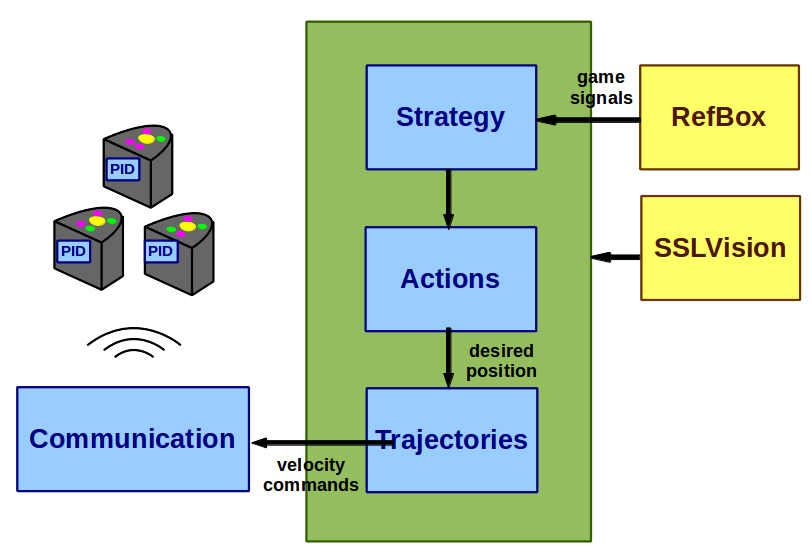
\includegraphics[width=12cm]{./pictures/eagle_knights_architecture.png}
	\caption{Eagle Knights SSL System Architecture}
	\label{fig:eagle-knights-architecture}  
\end{figure}

% \TODO{We need to update the diagram to include the monitor and any other node not in this diagram}


We have continued to evolve our robots' hardware to improve their performance. The on-board computing system is a Mojo V3 - FPGA and Microcontroller development board. We use Maxon 200142 brushless motors controlled through \textit{Afro} ESC's. We designed our own gear to reduce speed. Our communications use the XBee WiFi Module. Figure~\ref{fig:two-ekbots} shows two of our robots. The robot also have dribbler and kickers as shown in Figure~\ref{fig:ekbot-front}.

% \TODO{Include information about the kicker, validate that the information above is still valid}

\begin{figure}[htb]
	\centering
	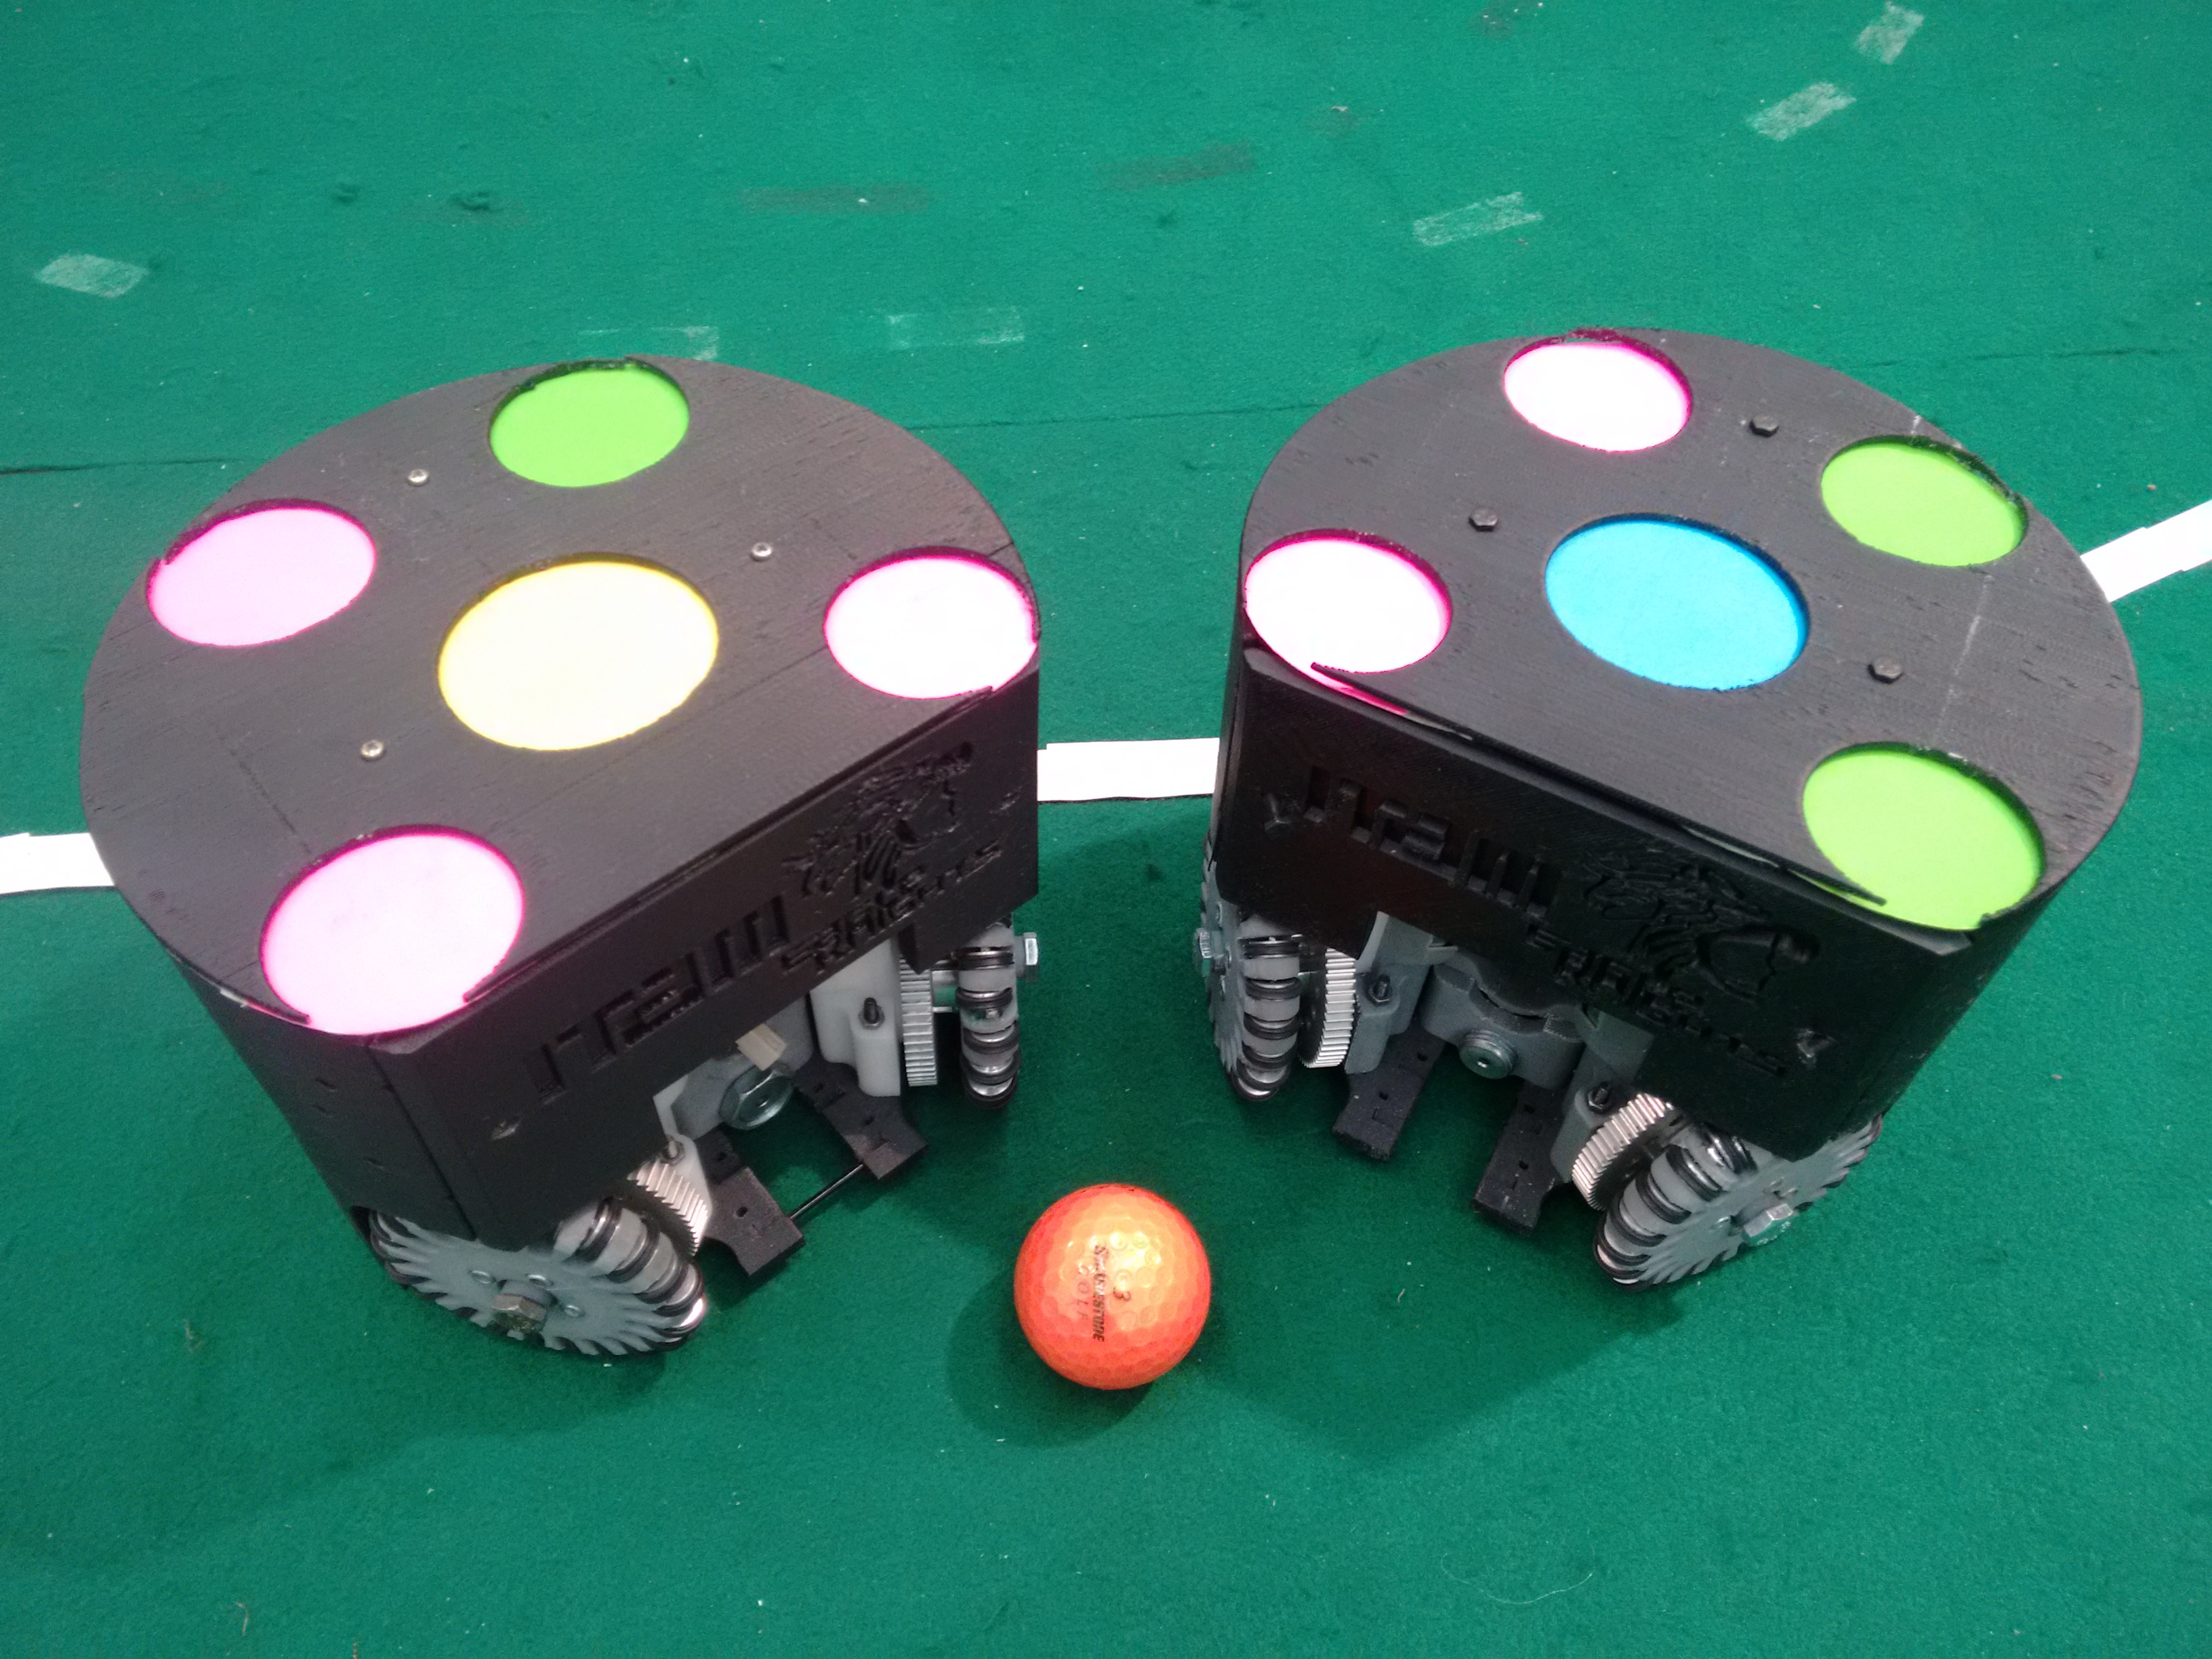
\includegraphics[width=6cm]{./pictures/two_ekbots.jpg}
	\caption{Eagle Knights SSL Robots}
	\label{fig:two-ekbots}  
\end{figure}

\begin{figure}[htb]
	\centering
	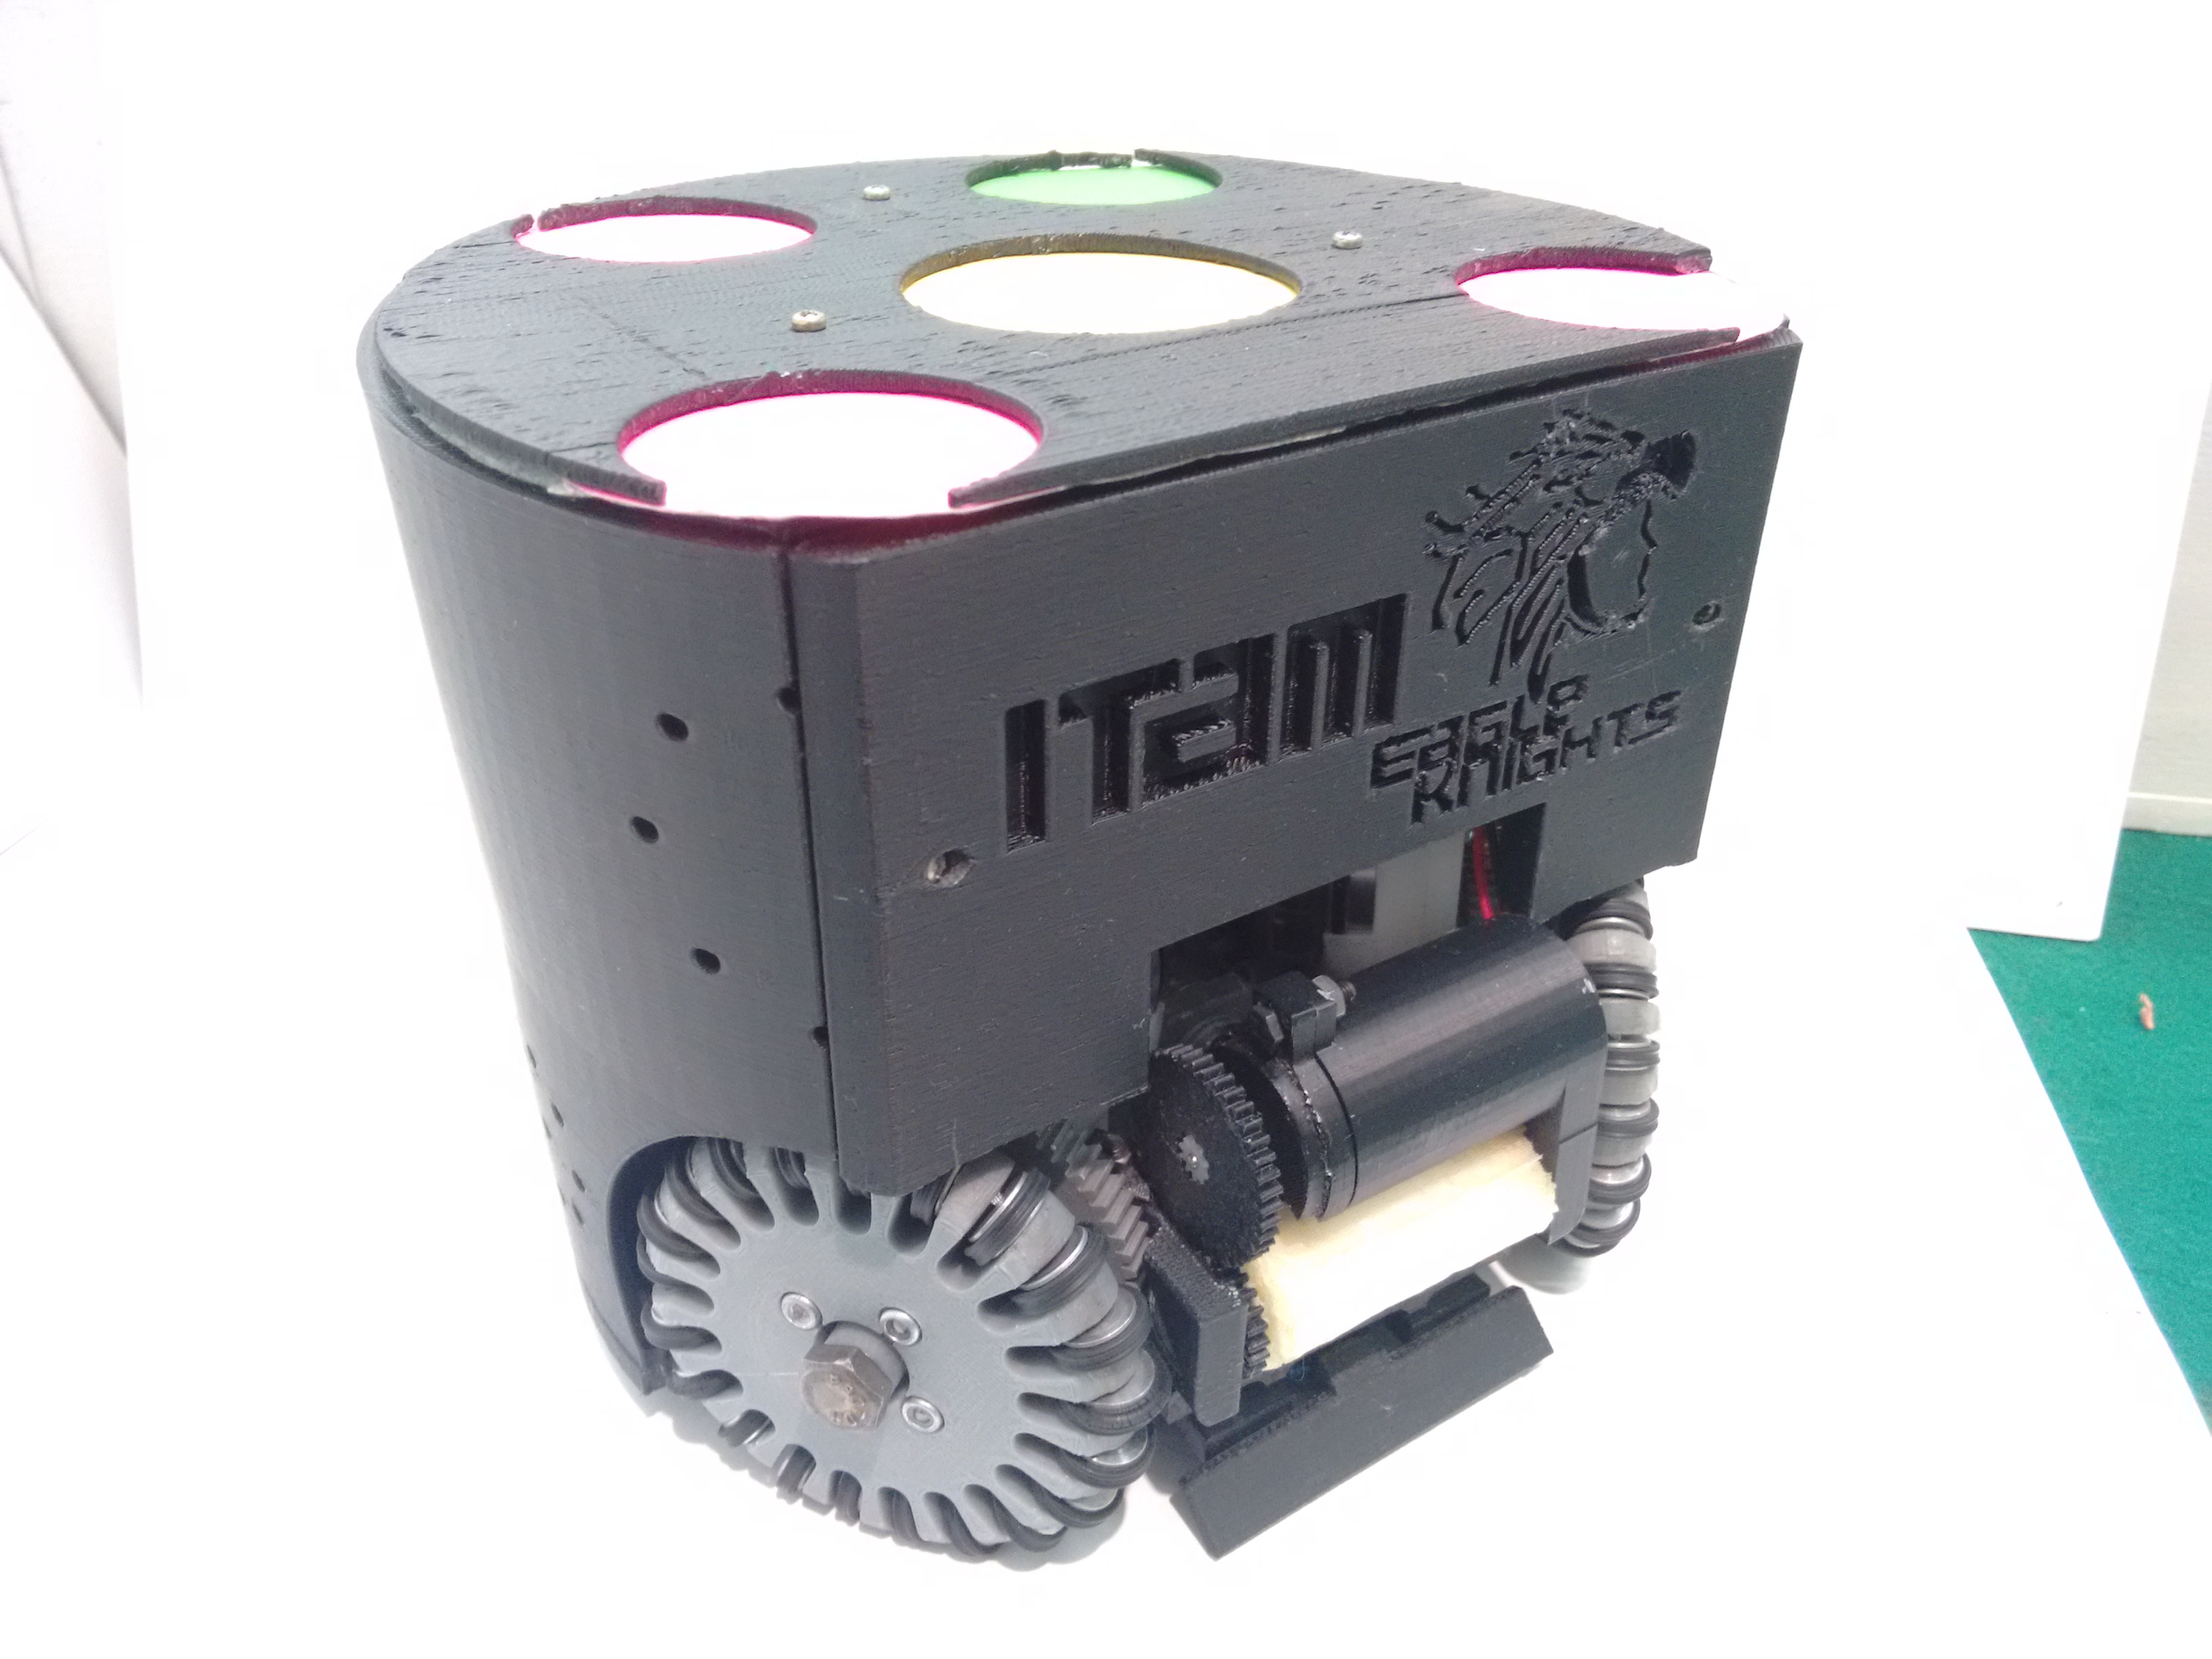
\includegraphics[width=6cm]{./pictures/ekbot_front.jpg}
	\caption{Eagle Knights SSL Robots}
	\label{fig:ekbot-front}  
\end{figure}

% \TODO{We probably need two pictures side by side, the current one and another from the front where the kicking system can be seen}



\section{ROS nodes}

We use the Robot Operating System (ROS) as the backbone of our system. It provides a framework to develop modular and distributed computation that has allowed us to produce compact modules that are easy to test and maintain. In ROS, we develop nodes that can communicate with each other through topics. Each node can provide its results as messages published to the appropriate topic. A node that needs a piece of information subscribes to the corresponding topic. Also, if using the right topics we can replace the robot with a robot simulator that allows us to test our algorithms even without real robots. Below, we describe each ROS node in our system.

\subsection{Monitor}
We have developed a Monitor with a GUI to track the robots, manual control and to display useful debugging output from the robots. 

% \TODO{We need to provide more information about the Monitor and its capabilities, with one example screenshot}
%\TODO{FUTURE: EKBots simulator}
%\TODO{FUTURE: User interface for setup}


\subsection{Referee Box}
A referee box node is a wrapper for the SSL referee box. This module controls the flow of the game, the robots are restricted to obey its commands. The Referee communicates the state of the game as decided by the referee. These messages are converted into ROS topics that are used by the role node, the action node, and the trajectory node.

% \TODO{verify if we need to mention anything concerning new rules. Perhaps logging ability?}

\subsection{Vision}
A vision node is a wrapper for the SSL vision system. For testing the Shared Vision System \cite{zlbwv-sslvtsvsftrcssl-RoboCup-2009} is used to digitally processes two video signals from the cameras mounted on top of the field. Its main tasks are to:
\begin{description}
	\item[Capture video] in real time from cameras mounted on top of the field.
	\item[Recognize] the colored patterns specified by the rules of the robots and ball. These patterns distinguish each robot and its team (yellow or blue) through 50-mm circular patches arranged in a unique way as defined in the rules of the SSL \cite{robocup-ssl-rules}. The ball is a standard orange golf ball.
	\item[Adapt] to different lighting conditions through color calibration.
	\item[Localize] the position and orientation of robots of both teams and the position of the ball.
\end{description}

In our current system we implemented a ROS client that produces a ROS topic per robot and another one for the ball. The Vision node produces messages at a rate of 30 Hz using the Pose2D type of message from the ROS geometry\_msgs library. Any other node can listen to the required topic depending on their specific task.
% \TODO{perhaps say a bit more about the structure of the topis, frequency of messages}
 


\subsection{Strategy}
A strategy node defines the actions for each player according to the state of the game, the role of the player, and the configurations of all the robots and of the ball. 

We currently support the following roles: goalkeeper and forward. Our strategies are very basic. The goalkeeper is always blocking the ball within the goal area. The forward follows the ball until it is close to it, and shoots towards the opposite goal.

% \TODO{verify this is what we do and update as necessary}

In the future we will apply motion planning and task planning techniques in order to identify better strategies.

\subsection{Action/Motion Planning}
An action/motion planning node defines the next position for each robot according to the action it is performing. Although several actions consist only of one move, some of them may include several distinct moves that are encoded as a state machine. At any given time, the action node produces a next position for the robot according to the active state machine. The actions that can be currently performed are: block ball, follow ball, and shoot ball. These are the action primitives:

\begin{description}
	\item[block ball] the robot moves to a point on the straight line between the robot and the ball depending on its role. If it is a goalie, it will move within the goal area, while if it is a defense, it will move outside the goal area.
	\item[follow ball] the robot moves to a point on the straight line between the robot and the ball within a small distance of the ball.
	\item[shoot ball] if the robot is far from the ball, it will move closer to the ball. If it is close to the ball, it will behind the ball on the straight line between the ball and the opposite team's goal. If it is already behind the ball, it will shoot the ball.
\end{description}

We also perform motion planning for avoiding other robots in the field either through potential functions \cite{k-rtoam-86} or through a geometric exploring tree (GET) \cite{eb-lppidewu-IEEEICMFI-1994}. Random points are produced and those within an obstacle are removed from the sample, using the remaining points, a path is find from the position of the robot to the desired position. 
% \TODO{explain how we perform motion planning for avoiding obstacles}

 
\subsection{Trajectory}
A trajectory node receives the current and goal configuration for each robot and computes the velocity command to be sent to them. This node takes in consideration the dynamic limitations of the robot to define a maximum acceleration and speed. We currently move in a straight line at constant speed between the start and the goal.

% \TODO{update if necessary}

\subsection{Communications}
A communications node receives velocity and action (dribbler and kicker) commands for the robots and passes them through a WiFi connection using UDP.




\section{Robots}

Figure~\ref{fig:one_ekbot_inside} shows some of the internal parts of our robots.

\begin{figure}[htb]
	\centering
	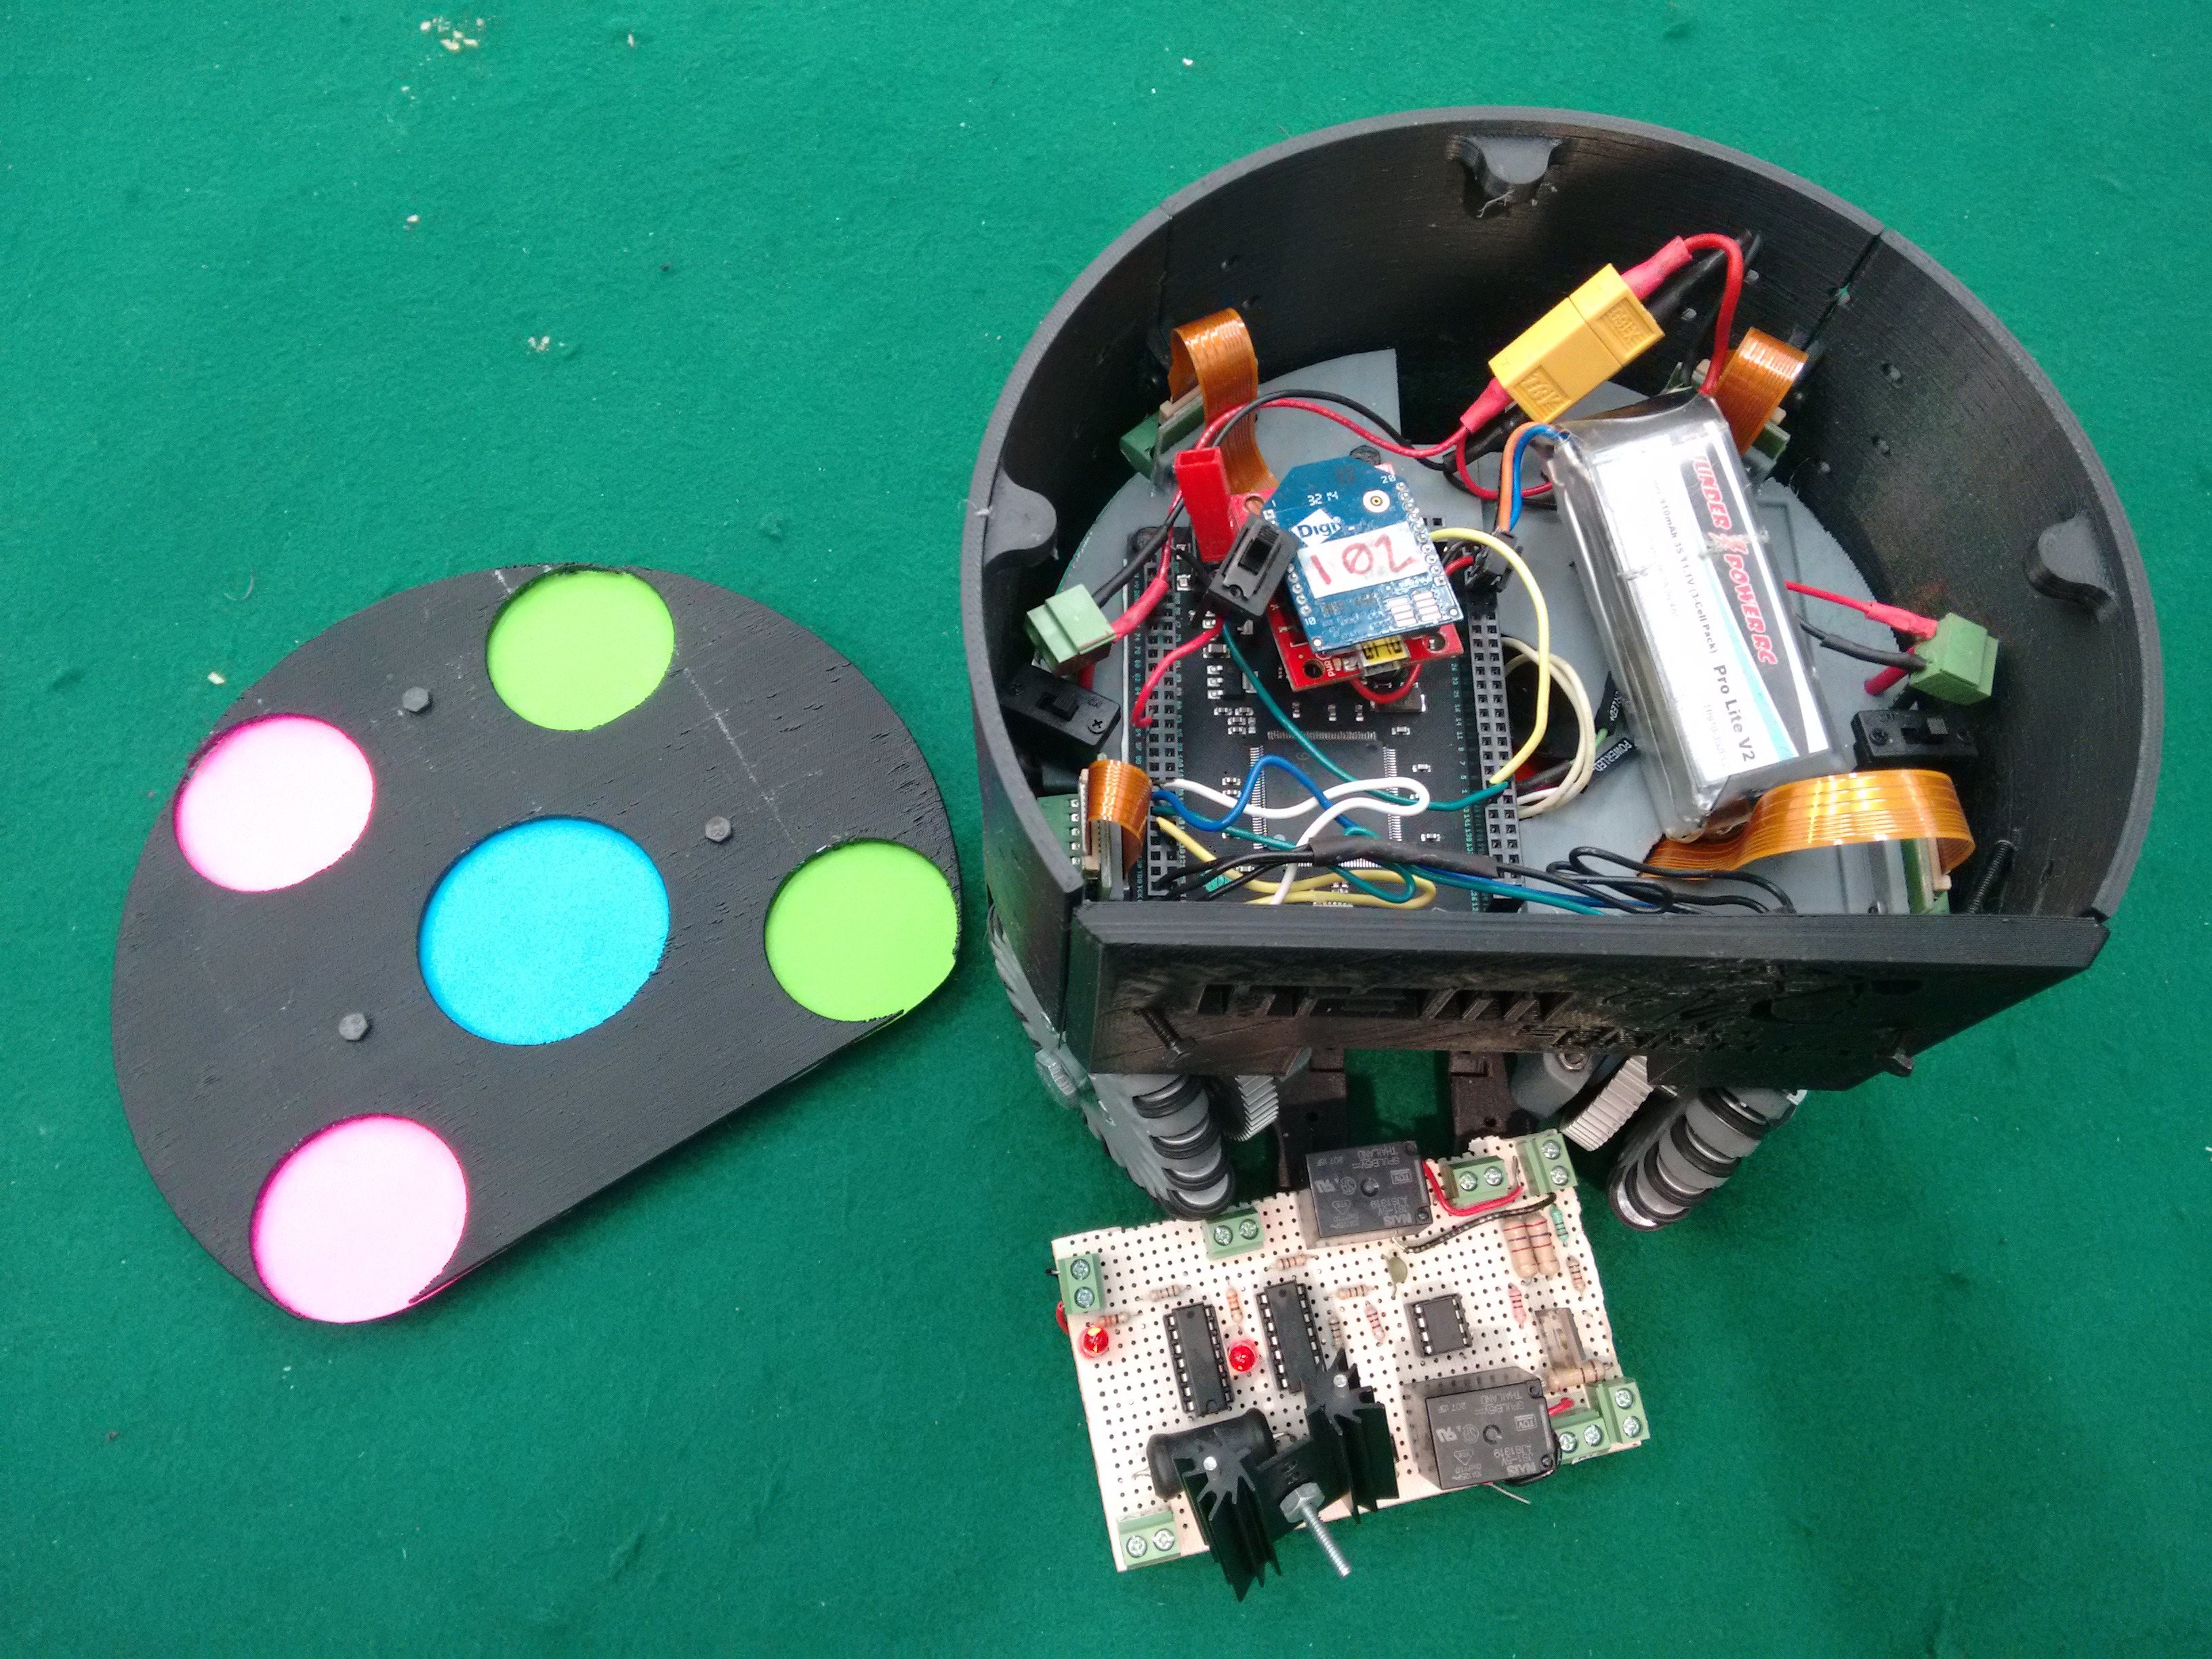
\includegraphics[width=6cm]{./pictures/one_ekbot_inside.jpg}
	\caption{Some internal parts of one of our robots}
	\label{fig:one_ekbot_inside}  
\end{figure}


\subsection{Robot Controller}
The robot performs on-board the kinematic computations to determine the speed for each motor. It also performs the computations for a PI algorithm for each motor using the information from the motor's sensors.  
% \TODO{Summary of the kinematic model of the robot and the PID control laws} 


\subsection{Omni-Directional Drive Micro-controller}
We use the Mojo V3-FPGA development board as our on-board computing system. Since it has an ARV ATMega32 micro-controller and a Spartan 6 FPGA, we can distribute computation in the robot itself. The micro-controller transforms the desired Cartesian speeds into motor speeds. Here we implemented a mapping from robot velocities (linear and angular) to motor velocities that are fed into a controller for each motor velocity. The micro-controller also handles a PI control algorithm for each motor. Simultaneously, the FPGA handles the actual control of each motor and reads the actual motor speeds to adjust the duty cycle of the PWM signals for each motor. The WiFi communication is handled by the FPGA. 


\subsection{Actuators}
Our robots have Maxon 200142 motors that run at an up to 4370 rpm. We have designed our own gear train with a reduction ratio of 3.5. We use a \textit{Afro} ESC for driving the motors. This allows our robots to move up to 3 m/s. Our kicker uses a low resistance solenoid.



\subsection{Kicker Control System}
Our kicker uses a push type solenoid. We have one 7.4V/ 700mA and two 11.1/900mA batteries. Since this amount of power is not enough to achieve minimum performance with the solenoid, we store energy through a voltage multiplier and discharge it when solenoid is activated. Activation happens when two conditions meet: a kicking signal is activated by the software, and an infrared sensor system in the bottom of the robot senses that the robot has the ball. 

\section{Research timeline for RoboCup 2017}
Since our last competition in RoboCup 2012, we continued with hardware improvements and we started our software from scratch. The current status of our system is that our robots can move in basic ways. We will be working in the following projects in order to get the system fully working by RoboCup 2017:

\begin{description}
	\item[Vision Node] We will complement our SSL Vision node with Kalman Filters to estimate future states of the ball and opposite robots.
	\item[Strategy Node] We currently only have a basic playing strategy. We will develop strategies for many more game situations than what we already have.
	\item[Action/Motion Planning Node] We will work intensely in having a good set of abilities for our robots.
	\item[Trajectory Node] Currently, our trajectories go at constant speed. We will try other approaches that handle better acceleration limits.
\end{description}


\section{Conclusions}

Here we described our robotic soccer team in order to participate in RoboCup 2017. Our current capabilities are basic, however we plan to have a team able to play by the time of the competition. Also, we have a long-term plan with the goal of having a competitive team with two years. 

% \TODO{Write something about performance}


\section{Acknowledgements}
This work is supported by the Asociación Mexicana de Cultura, A.C. and the Instituto Tecnológico Autónomo de México.

\bibliographystyle{unsrt}
\bibliography{robocup,robotics}


\end{document}
